\chapter{Projektformulering}




\textbf{Ansvarsområde} \\
Projektets opgaver er blevet uddelt mellem nedenstående seks gruppemedlemmer. En gruppe har haft ansvaret for udvikling hardware og dokumentering heraf, og en anden gruppe har haft ansvar for udvikling af software, samt en ligeledes dokumentering heraf. 



\begin{longtabu} to \linewidth{@{}  l X[j]@{}}
    Område &    Ansvarlig\\[-1ex]
    \midrule
	Hardware-udvikling og dokumentation & FRM, NHL og SSK\\
	Software-udvikling og dokumentation & JTH, TSN og MFJ \\
	Resterende rapportafsnit & Alle\\
	\caption{Ansvarsområder}
	\label{Ansvar}
\end{longtabu}

\textbf{Initialer: } \\
Jeppe Tinghøj Honoré - JTH \\
Mads Fryland Jørgensen - MFJ \\
Tine Skov Nielsen - TSN \\
Freja Ramsing Munk - FRM \\
Nicoline Hjort Larsen - NHL \\
Sara-Sofie Staub Kirkeby - SSK \\[2ex]

\textbf{Projektformulering}\\
I dette projekt var problemstillingen at lave en invasiv blodtryksmåler til en valgfri institution. Der er i den forbindelse blevet arbejdet med blodtryksmåling, udvikling af hardware til blodtryksmåleren samt udarbejdelse af et program til analyse af blodtryksmålingen.\\ 
\\
Motivationen for projektet bygger på, at der i klinisk praksis ofte er behov for kontinuert at kunne monitorerer en patients blodtryk. Dette er især vigtigt på en operationsstue, hvor blodtrykket er en vigtig parameter til monitorering af patientens helbredstilstand, hvilket også ligger til grund for udarbejdelsen af dette projekt.\\
\begin{figure}[H]
	\centering
	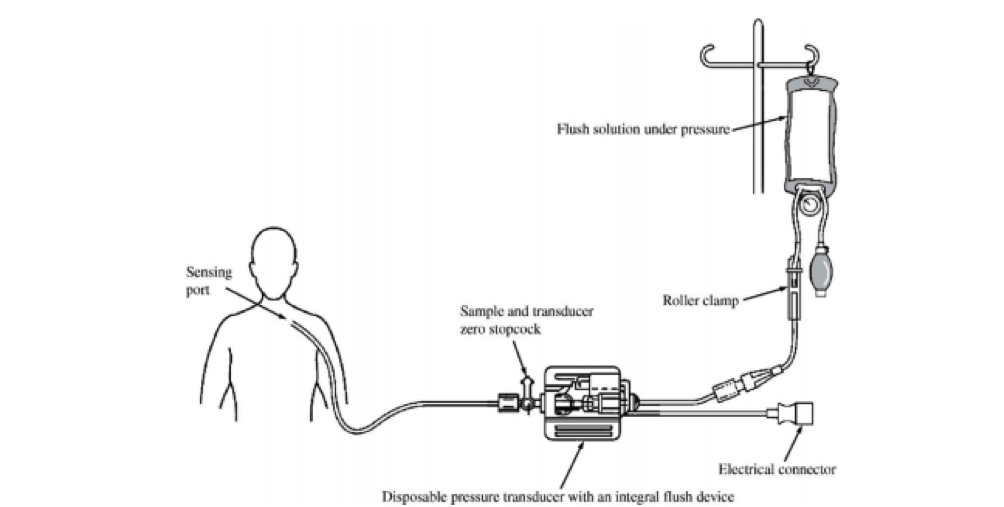
\includegraphics[width=0.8\textwidth]{Figurer/Indledning/Opstilling}
	\label{Opstilling}
	\caption{Tilslutningen af væskefyldt kateter}
\end{figure}
Da det er vigtigt med kontinuerlige målinger af blodtrykket, bliver målingen foretaget invasivt. På billedet ses det, hvordan blodtryksmålesystemet er tilsluttet patientens arterier via et væskefyldt kateter.\\ 
I dette projekt skal der arbejdes på at udarbejde et system, der kan tilsluttes det væskefyldte kateter og vise en blodtrykskurve, samt blodtryksværdier på en computerskærm. \\
Systemet skal bestå af to elementer:
\begin{enumerate}
	\item Det ene element består af et elektronisk kredsløb, der forstærker signalet fra transduceren og filtrerer signalet med et indbygget analogt filter.
	\item Det andet element er et program, der afbilder blodtrykket grafisk som funktion af tiden. Programmet skal ligeledes vise blodtryksværdier, samt puls og kunne udløse en alarm, hvis grænseværdier for blodtrykket overskrides. 
\end{enumerate}
\textbf{Afgrænsning}\\ \\
Fra IHA’s side er der på forhånd defineret nogle krav til projektets indhold, hvilket indebærer:\\ \\
Hardware
\begin{itemize}
	\item Der skal designes et aktivt 2. ordens lavpasfilter af typen Sallen-Key med unity gain
	\item Filteret skal designes som et Butterworth-filter med cutoff-frekvens på 50Hz. C2 skal vælges til 680nF og R1 = R2. Operationsforstærkeren skal være af typen OP27
\end{itemize}
Software 
\begin{itemize}
	\item Programmet skal programmeres i C\#
	\item Programmet skal kunne kalibrere blodtrykssignalet og foretage en nulpunktsjustering
	\item Programmet skal kunne vise blodtrykssignalet kontinuerligt
	\item Programmet skal kunne lagre de målte data i enten en tekstfil eller en database
	\item Programmet skal kunne filtrere blodtrykket i selve programmet via et digitalt filter, hvilket skal kunne slås til og fra
\end{itemize}


Projektets resultat vil kunne hjælpe sundhedsfagligt personale med at bevare overblikket over deres patients fysiske tilstand under en operation. Da det både kan være en planlagt eller akut situation på operationsstuen er det vigtigt, at systemet virker optimalt og udøver den bedste hjælp til personalet.
